\section{Betrachtungsgegenstand}
Der derzeitige State-Of-The-Art im Bereich \ac{T2P} ist das Verfahren von Friedrich aus dem Jahr 2011 (\cite[vgl.][11]{RIEFER}). Im Folgenden wird die von Friedrich erarbeitete Vorgehensweise (\cite[vgl.][]{FRIEDRICH1} und \cite[vgl.][]{FRIEDRICH2}) analysiert und Verbesserungsvorschläge erarbeitet. Die Analyse beschränkt sich auf die Textverarbeitung und die daraus resultierende Generierung des World Models (Text-2-WorldModel). Die Konstruktion eines Graphen (Text-2-BPM) aus dem World Model ist nicht Teil dieser Arbeit.
\par
Zunächst wird im Folgenden kurz auf den konkreten Aufbau des World Models nach Friedrich eingegangen. Anschließend folgt die Analyse der Vorgehensweise. Gemäß der durch Friedrich vorgegebenen Gliederung wird zunächst die Textverarbeitung auf Satz-Ebene und dann die Textverarbeitung auf Text-Ebene analysiert. Abschließend werden bekannte Problemfelder zusammengetragen und Lösungsansätze vorgeschlagen.

\section{World Model}
Die Verwendung einer World-Model-Datenstruktur als Zwischenspeicher für die aus einem Text extrahierten Informationen ist in diesem Umfeld üblich. Friedrich greift auf bestehende Ansätze zurück und modifiziert die Datenstruktur, sodass später ein \ac{BPMN}-Graph abgeleitet werden kann.Das World Model nach Friedrich beinhaltet 8 Klassen (\cite[vgl.][46]{FRIEDRICH2}). 
\par
\begin{itemize} 
\item ORIGINATED ELEMENT: Aus einem Text extrahierte Entität. Um Rück\-ver\-folg\-bar\-keit zu ermöglichen wird hier eine Referenz zum Ursprungssatz hinterlegt.
\item SPECIFIED ELEMENT: Verfeinerung des \textit{Originated Element}. Speicher einen Bezug zu einem Wort im Text und wird genutzt um mit \textit{Specifiern} zu interagieren.
\item SPECIFIER: Annotierte Information, die zur genaueren Spezifikation eines \textit{Specified Element} dient.
\item EXTRACTED OBJECT: Textpart, der vom Hauptsatz extrahiert wurde. Es erbt vom \textit{Specified Element} und wird  von \textit{Actor} und \textit{Resource} genauer spezifiziert.
\item ACTOR: Subjekt eines Satzes, das als agierende Entität zu verstehen ist. 
\item RESOURCE: Objekt eines Satzes.
\item ACTION: Aus dem Text extrahierte Aktivität, die einen \textit{Actor} und eine \textit{Resource} besitzen kann. Eine Aktivität kann mit weiteren Aktivitäten verbunden werden.
\item FLOW: Repräsentiert die Beziehungen zwischen Aktivitäten. Es wird zwischen den beiden Möglichkeiten \textit{Split-Flow} und \textit{Join-Flow} unterschieden. Darüber hinaus spezifiziert der Typ, ob es sich um gleichzeitige, sequenziell ablaufende, Entscheidungs- oder Ausnahme-Relationen handelt.
\end{itemize}

Der korrekte Aufbau dieses World Models aus dem Text ist Grundvoraussetzung für die erfolgreiche Erstellung eines Graphen. Es entsteht Schritt für Schritt durch die folgenden Verarbeitungsschritte.

\section{Textverarbeitung auf Satz-Ebene}

Der Eingangstext in natürlicher Sprache wird zunächst in einzelne Wörter und Sätze aufgesplittet. In Abbildung \ref{fig:SLEVEL} wird dieser Vorgang der \textit{Sentence Decomposition} zugeordnet. Es handelt sich hierbei um eine normale Tokenization, bei der auf die Stanford CoreNLP Funktionen \textit{Stanford TokenizerAnnotator} und \textit{Stanford WordsToSentenceAnnotator} zurückgegriffen wird. Im nächsten Schritt wird der Text mit dem \textit{POSTaggerAnnotator} mit \textit{POS-Tags} versehen und anschließend mit dem PCFG-Parser \textit{ParserAnnotator} die Satzstruktur analysiert. Dies wird durch den Pfeil von StanfordParser zu Subprozess in Abbildung \ref{fig:SLEVEL} symbolisiert. Auf eine pauschale \textit{Lemmatization} aller Wörter wird an dieser Stelle verzichtet. Die zwei weiteren an dieser Stelle üblichen Standard-Analysemöglichkeiten \textit{Collocation Extraction} (Erkennen von zusammengesetzten Wörtern) und \textit{Named Entity Recognition} (Analyse von Eigennamen) werden ebenfalls nicht genutzt.\par

\begin{figure}[H]
\begin{center}
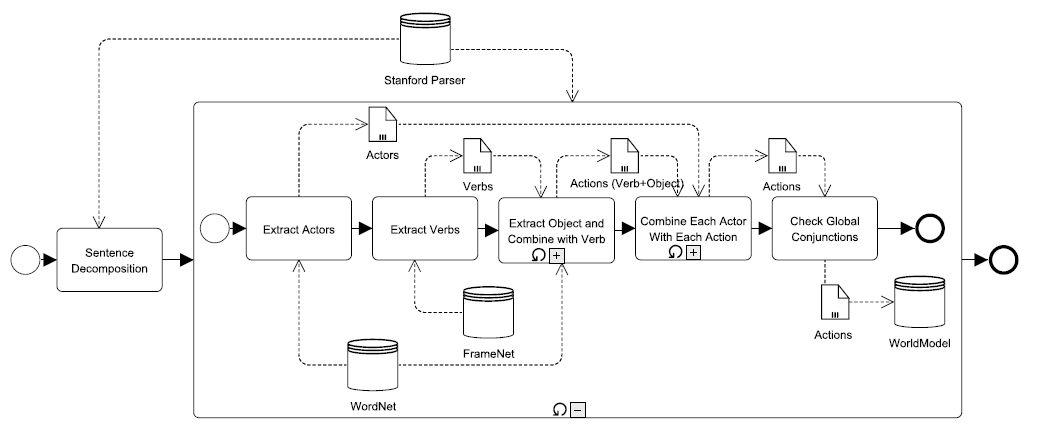
\includegraphics[keepaspectratio=true, width=\textwidth]{pictures/SentenceLevel.png}
\caption{Analyseschema auf Satzebene (\cite[vgl.][5]{FRIEDRICH2})}
\label{fig:SLEVEL}
\end{center}\end{figure}
Auf Basis der Annotationen folgt dann das \textit{Phrase Chunking}, der zweite Teil der Sentence Decomposition. Hierzu analysiert ein von Friedrich selbst entwickelter Algorithmus die Informationen zur Satzstruktur (\cite[vgl.][49]{FRIEDRICH2}). Haupt-und Nebensätze werden identifiziert und  auf Abhängigkeiten untersucht. Nebensätze werden als irrelevant klassifiziert und herausgefiltert, wenn keine Abhängigkeit zum Hauptsatz besteht. Relativsätze werden zunächst ignoriert.
\par
Der in \ref{fig:SLEVEL} dargestellte Subprozess wird von Friedrich als \textit{Element Extraction} bezeichnet und umfasst die semantische Analyse auf Satz-Ebene. Zunächst wird der Actor aus dem Satz extrahiert. Bei einem Satz im Aktiv, wird hierfür nach einem Specified Object mit dem Specifier \textit{nsubj} \footnote{Eine kurze Erläuterung der Stanford-Dependency-Kürzel findet sich hier: https://nlp-ml.io/jg/software/pac/standep.html} gesucht. Bei einem Satz im passiv nach einem Specified Object mit Specifier \textit{agent}. Wird ein Actor gefunden, kann ein Actor-Objekt erstellt, mit Zusatzinformationen über mögliche logische Konjunktionen versehen und in einer Liste gespeichert werden. Als nächstes wird die Action identifiziert.  Eine Action ist im Gegensatz zu einem Actor nicht optional. Eine Action basiert immer auf einem Verb. Dieses findet sich entweder über die \textit{nsubj}-, die \textit{cop}- oder die \textit{dobj}-Beziehung. Bei Sätzen im Passiv ist die \textit{nsubjpass}-Relation Aufschluss gebend. Auf vergleichbare Art werden die zum Verb gehörenden Objekte extrahiert und mit Hilfe von WordNet als Actor oder Resource klassifiziert. Anschließend werden zum Verb gehörende Relativsätze analysiert und dann alles mit Zusatznformationen über mögliche logische Konjunktionen und in einer zweiten Liste gespeichert. Die Identifikation und Handhabung von logischen Konjunktionen \footnote{Logische AND-Verknüpfungen wie beispielsweise in: \textit{He reads AND drinks coffee.}} erfolgt ebenfalls mittels eines eigenen Algorithmus. Im letzten Schritt des Subprozesses erfolgt die Speicherung der Informationen im Worldmodel.
\par
Die Identifikation der semantischen Rollen erfolgt hier folglich komplett regelbasiert über die Syntax-Annotationen mittels eines von Friedrich entwickelten Algorithmus. Zwar wird FrameNet eingesetzt, um Objekten auf Basis ihres Beszugsverbes ein Frame Element zuzuordnen, doch auf ein bestehendes \ac{SRL} Tool wird nicht zurückgegriffen. Die Klassifikation eines Objektes als Actor oder Resource mittels WordNet könnte durch Named Entity Recognition und einen Word-Sense-Disambiguation-Algorithmus verbessert werden.

\section{Textverarbeitung auf Text-Ebene}
\label{subsec:TextLevel}

\begin{figure}[H]
\begin{center}
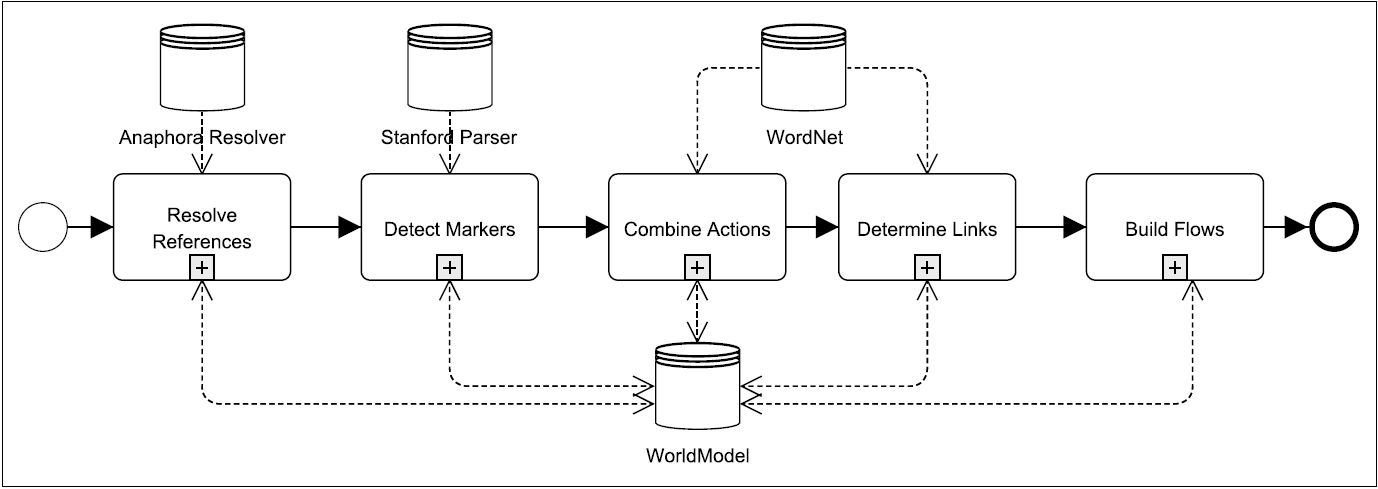
\includegraphics[keepaspectratio=true, width=\textwidth]{pictures/textLevel.png}
\caption{Analyseschema auf Textebene (\cite[vgl.][7]{FRIEDRICH2})}
\label{fig:TLEVEL}
\end{center}\end{figure}

Die Analyse auf Text-Ebene erfolgt in 5 Schritten, wie Abbildung \ref{fig:TLEVEL} zeigt. Der erste Schritt hierbei ist die Auflösung von Beziehungen über Pronomen zwischen den Sätzen. Friedrich definiert zu diesem Zweck einen Algorithmus mit der Bezeichnung \textit{Anaphora Resolver}, welcher auf den Stanford Parser aufbaut (\cite[vgl.][67 ff.]{FRIEDRICH1}). Allerdings ist eine solche Funktionalität mittlerweile auch Bestandteil des Stanford CoreNLP Kits, wie in Abschnitt \ref{subsec:coref} erläutert wurde. Der Schritt der Auflösung der Beziehungen könnte folglich bei zukünftigen Implementierungen mit Anwendung des CoreNLP Kits als ausgelagert betrachtet werden.\par
Der nächste Schritt ist die Ermittlung aller \textit{Marker}. Diese bezeichnen nach Friedrich eine bestimmte Menge von Wörten und Phrasen, die jeweils bestimmte Operatoren bei der \ac{BPMN} repräsentieren. Dabei werden 4 verschiedene Klassen differenziert:  Bedingungsindikatoren, Parellelitätsindikatoren, Ausnahmeindikatoren und Folgeindikatoren. Für jede dieser Klassen wird als heuristischer Ansatz eine statische Menge von entsprechenden Ausdrücken in natürlicher Sprache als Referenz verwendet, die aus Testdaten extrahiert wurden. Auf Basis dieser Mengen wird ein Algorithmus angewandt, der anhand der Ergebnisse des Stanford Parsers derartige Marker identifiziert. Problematisch hierbei ist, dass Marker in vielen grammatikalischen Varianten und teils auch implizit vorkommen können (\cite[vgl.][73 ff.]{FRIEDRICH1}).\par
Anschließend werden die Actions ermittelt, die über mehrere Sätze beschrieben wurden. Durch Schritt 1 wurden bereits Beziehungen zwischen Sätzen ermittelt. Diese dienen als Basis für die Ermittlung kombinierter Actions. Alle Actions, die mit einem anderen Satz in Verbindung stehen gelten als Kandidaten für kombinierte Actions. Diese werden nach verschiedenen Bedingungen geprüft. Eine Bedingung ist, dass eine der beiden Actions als \textit{weak action}, also als unselbstständige Action, kategorisiert werden kann. Diese Kategorisierung wird mithilfe von WordNet durchgeführt. Treffen die definierten Bedingungen zu, werden die beiden Actions zu einer einzigen vereinigt (\cite[vgl.][77 ff.]{FRIEDRICH1}).\par
Ein weiterer Schritt ist die Analyse von Bezügen zwischen den Actions. Es werden Vorwärts-, Rückwärts- und Sprungbezüge unterschieden. In diesem Zuge werden alle Actions jeweils miteinander verglichen. Mithilfe der \textit{Lemmata} aus Wordnet werden so die einzelnen Eigenschaften der Actions in Bezug auf Analogien evaluiert. Ähneln sich die verglichenen Actions nach bestimmten Kriterien, wird ein Bezug im World Model erstellt (\cite[vgl.][82 ff.]{FRIEDRICH1}).\par
Letztlich werden auf Basis aller Informationen die Flows generiert. Es wird davon ausgegangen, dass der Text den Prozess sequentiell beschreibt (\cite[vgl.][83 ff.]{FRIEDRICH1}).


\section{Problemfelder und Lösungsansätze}
Die Evaluation des State-Of-The-Art Ansatzes anhand von Testdaten ergab, dass durchschnittlich 76\% eines Modells korrekt erzeugt werden kann (\cite[vgl.][115]{FRIEDRICH1}). Ebenfalls ergibt sich aus der Evaluation, welche Problemfelder bei diesem Ansatz bestehen.\par Zum einen sinkt die Korrektheit der erzeugten Modelle mit steigender Länge des analysierten Textes. Dies hat damit zutun, dass die Erkennung von Meta-Sätzen und für den Prozess irrelevanten Informationen problematisch ist (\cite[vgl.][116]{FRIEDRICH1}). Behandelt wird dieses Problem mit den in Abschnitt \ref{subsec:TextLevel} dargelegten Maßnahmen. Diese Beruhen im Wesentlichen auf der Coreference Resolution. Die Verwendung der im Vergleich präziseren Coreference Resolution des Stanford CoreNLP Kits könnte sich daher positiv auf dieses Problem auswirken.\par
Außerdem ist nach Friedrich auch die Genauigkeit und Funktionsweise der Tools ein Problem. So liefert der Stanford Parser beispielsweise häufig nicht die Klassifikation der Verben (\cite[vgl.][117 ff.]{FRIEDRICH1}). Da allerdings mittlerweile eine neue Implementierung dessen existiert, wie in Abschnitt \ref{subsec:parser} dargelegt, muss diese Aussage neu evaluiert werden.\par
Zusammenfassend ergibt sich, dass ein Update des State-Of-The-Art Ansatzes mit aktuelleren \ac{NLP} Tools sich positiv auf dessen bestehende Probleme auswirken könnte.


